% SPDX-License-Identifier: AGPL-3.0-or-later
% SCAHI method overview (TikZ). Build: lualatex fig_method.tex  (images from ../assets, colours = paper figure palette)
\documentclass[tikz,border=4pt]{standalone}
\usepackage{amsmath}
\usepackage{fontspec}
\usepackage{unicode-math}
\setmainfont{Inter}[Scale=0.92]
\setmathfont{Fira Math}[Scale=0.92]
\hyphenpenalty=10000 \exhyphenpenalty=10000
% math spacing without stretch: nodes with a fixed text width otherwise stretch the space around = (user 2026-11-05)
\thickmuskip=5mu\relax \medmuskip=4mu\relax
\usepackage{pgfplots}
\pgfplotsset{compat=1.18}
\usetikzlibrary{positioning,arrows.meta,calc,fit,backgrounds,shapes.geometric,decorations.pathreplacing}
\graphicspath{{../assets/}}

% SPDX-License-Identifier: AGPL-3.0-or-later
% generated by scripts/figstyle.py - do not edit (colours of the matplotlib figures)
\definecolor{ink}{HTML}{0B0B0B}
\definecolor{ink2}{HTML}{52514E}
\definecolor{muted}{HTML}{8A8984}
\definecolor{grid}{HTML}{E3E2DC}
\definecolor{blue}{HTML}{2A78D6}
\definecolor{bluel}{HTML}{CDE2FB}
\definecolor{bluem}{HTML}{86B6EF}
\definecolor{blued}{HTML}{184F95}
\definecolor{orange}{HTML}{EB6834}
\definecolor{orangel}{HTML}{FBE1D6}
\definecolor{aqua}{HTML}{1BAF7A}
\definecolor{panel}{HTML}{F6F6F3}
  % colours from scripts/figstyle.py

\tikzset{
  >={Stealth[length=2.2mm]},
  lab/.style={font=\scriptsize\bfseries, text=ink, align=center},
  sub/.style={font=\tiny, text=ink2, align=center},
  box/.style={draw=ink2, line width=0.5pt, rounded corners=2pt, fill=white, align=center, font=\scriptsize, text=ink,
              inner sep=3pt},
  mbox/.style={box, draw=blue, line width=0.8pt},
  bbox/.style={box, draw=orange, line width=0.8pt},
  flow/.style={->, line width=0.9pt, draw=blue},
  bflow/.style={->, line width=0.9pt, draw=orange},
  stage/.style={font=\tiny\bfseries, text=muted},
}

\begin{document}
\begin{tikzpicture}[x=1cm, y=1cm]

% main flow on one horizontal axis y = 0 (centre of the image): every connector of the main path is horizontal
% ---------------------------------------------------------------- (1) input
\node[inner sep=0, draw=ink2, line width=0.4pt] (img) at (0,0) {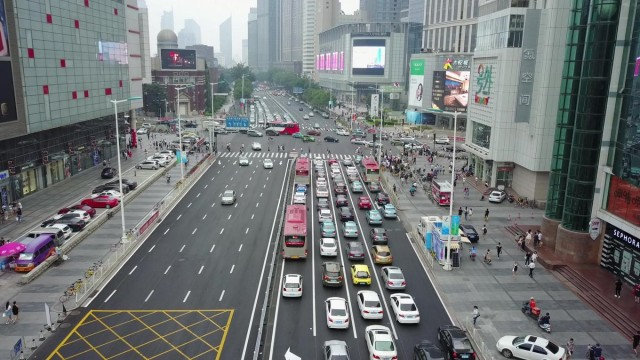
\includegraphics[width=2.5cm]{input.jpg}};
\node[lab, above=1mm of img] {Image $I$};
\node[sub, below=0.5mm of img] {$1360\times765$ (VisDrone)};

% ---------------------------------------------------------------- (2) zoom stack
\node[inner sep=0, draw=ink2, line width=0.4pt, right=9mm of img, yshift=8.905mm] (z0) {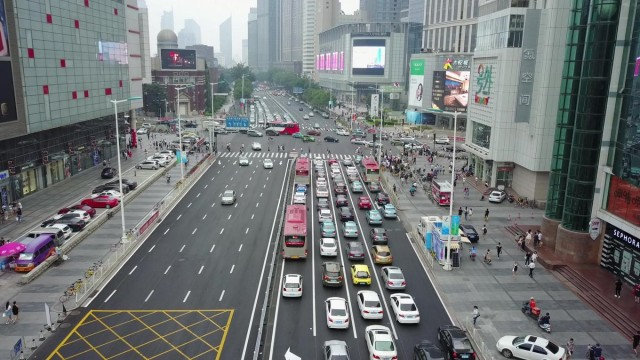
\includegraphics[width=2.1cm]{input.jpg}};
\node[inner sep=0, draw=ink2, line width=0.4pt, below=6mm of z0] (z2) {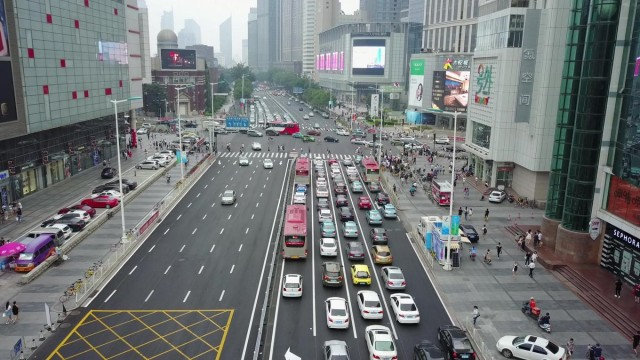
\includegraphics[width=2.1cm]{input.jpg}};
% tile grid of the z = 2 level (T = 512 px of 1360 x 765, overlap 0.3) drawn over the thumbnail
\begin{scope}[shift={(z2.south west)}, x=2.1cm/1360, y=2.1cm/1360]
  \foreach \x in {0,358,716,848} { \draw[white, line width=0.45pt, dash pattern=on 1.4pt off 1.1pt] (\x,0) rectangle ++(512,512); }
  \foreach \x in {0,358,716,848} { \draw[white, line width=0.45pt, dash pattern=on 1.4pt off 1.1pt] (\x,253) rectangle ++(512,512); }
  \draw[blue, line width=0.9pt] (424,40) rectangle ++(512,512);
\end{scope}
\node[sub, right=0.5mm of z0, anchor=west, text width=1.5cm, align=left] {whole image\\at train size\\(e.g.\ 1280 px)};
\node[sub, right=0.5mm of z2, anchor=west, text width=1.5cm, align=left] {$z{=}2$: tiles\\$T{=}N/z{=}512$ px\\$\to N{=}1024$};
\node[lab, above=1mm of z0] {Zoom stack};
\draw[flow] (img.east) -- ++(4mm,0) |- (z0.west);
\draw[flow] (img.east) -- ++(4mm,0) |- (z2.west);

% ---------------------------------------------------------------- (3) detector
\node[trapezium, trapezium angle=72, shape border rotate=270, draw=blue, line width=0.8pt, fill=bluel!35, minimum height=1.9cm,
      minimum width=1.1cm, anchor=west, at={($(z0.east|-img.center)+(23mm,0)$)}, font=\scriptsize, align=center, text=ink] (det)
      {dense\\detector\\[-1pt]{\tiny (e.g.\ YOLOv10s)}\\[-1pt]{\tiny shared}\\[-3pt]{\tiny across}\\[-3pt]{\tiny passes}};
\node[lab, above=1mm of det] {Detector};
\coordinate (zm) at ($(z0.east|-img.center)+(19mm,0)$);
\draw[line width=0.9pt, draw=blue] (z0.east) ++(15.5mm,0) -| (zm);
\draw[line width=0.9pt, draw=blue] (z2.east) ++(15.5mm,0) -| (zm);
\draw[flow] (zm) -- (det.west);

% ---------------------------------------------------------------- (4) dense per-position outputs (cache); both paths branch here
\begin{scope}[shift={($(det.east)+(9mm,-6mm)$)}]
  \foreach \k/\c in {0/bluel, 1/bluel!70, 2/bluel!45} {
    \begin{scope}[shift={(0.12*\k,0.12*\k)}]
      \fill[\c, draw=blue!70, line width=0.35pt] (0,0) rectangle (1.1,1.1);
      \foreach \i in {0.22,0.44,...,0.9} { \draw[blue!35, line width=0.2pt] (\i,0) -- (\i,1.1); \draw[blue!35, line width=0.2pt] (0,\i) -- (1.1,\i); }
    \end{scope}
  }
  \foreach \p/\s in {{0.3,0.5}/1.6, {0.75,0.8}/1.1, {0.6,0.3}/1.9, {0.9,0.45}/0.9} { \fill[blue] (\p) circle (\s pt); }
  \coordinate (rawc) at (0.6,0.6);
  \node[lab, text width=2.6cm] at (0.66,-0.32) {Dense per-position\\outputs};
  \node[sub, text width=2.2cm] at (0.66,-0.98) {per pass \& position:\\$(x,y,\sigma,\,p_c)$, $p\ge10^{-3}$\\(cached)};
\end{scope}
\draw[flow] (det.east) -- ($(rawc)+(-0.62,0.0)$);

% ---------------------------------------------------------------- (5) windows
\begin{scope}[shift={($(rawc)+(1.75,-0.525)$)}]
  \node[lab, anchor=south] at (1.05,1.2) {Border taper};
  \begin{axis}[at={(0,0.15cm)}, width=2.1cm, height=0.75cm, scale only axis, axis lines=left, xmin=0, xmax=10, ymin=0, ymax=1.15,
      xtick=\empty, ytick=\empty, axis line style={draw=muted, line width=0.4pt}, clip=false,
      every axis plot/.append style={line width=0.8pt}]
    \addplot[domain=0:4, samples=40, blue] {x<1.2 ? sin(deg(pi/2*x/1.2))^2 : (x>2.8 ? sin(deg(pi/2*(4-x)/1.2))^2 : 1)};
    \addplot[domain=2.8:7.2, samples=40, bluem] {x<4 ? sin(deg(pi/2*(x-2.8)/1.2))^2 : (x>6 ? sin(deg(pi/2*(7.2-x)/1.2))^2 : 1)};
    \addplot[domain=6:10, samples=40, blued] {x<7.2 ? sin(deg(pi/2*(x-6)/1.2))^2 : 1};
    \addplot[domain=0:10, samples=2, ink, dashed, line width=0.5pt] {1};
    \node[sub, anchor=north] at (axis cs:5,-0.02) {border $b_t(x)$};
  \end{axis}
  \node[sub, anchor=north, text width=2.4cm] at (1.05,-0.35) {weight $\omega=b_t$: border taper\\of tile $t$ only};
  \coordinate (winc) at (1.05,0.525);
\end{scope}
\draw[flow] ($(rawc)+(0.75,0)$) -- ($(winc)+(-1.18,0)$);

% ---------------------------------------------------------------- (6) scale-space volume
\begin{scope}[shift={($(winc)+(1.75,-1.15)$)}]
  \node[lab] at (1.25,2.95) {Scale space $F(x,y,\log\sigma)$};
  \foreach \k/\g/\c in {0/0.14/bluel!55, 1/0.22/bluel!75, 2/0.36/bluel} {
    \begin{scope}[shift={(0.18*\k,0.78*\k)}, yslant=0.0, xslant=0.55]
      \fill[\c, draw=blue!65, line width=0.35pt, opacity=0.92] (0,0) rectangle (1.75,0.62);
      \pgfmathsetmacro{\gg}{2*\g}
      \begin{scope}
        \clip (0,0) rectangle (1.75,0.62);
        \foreach \i in {\g,\gg,...,1.7} { \draw[blue!35, line width=0.18pt] (\i,0) -- (\i,0.62); }
        \foreach \j in {\g,\gg,...,0.6} { \draw[blue!35, line width=0.18pt] (0,\j) -- (1.75,\j); }
      \end{scope}
    \end{scope}
  }
  \fill[blued] (0.95,0.33) circle (1.6pt); \fill[blued] (1.62,1.12) circle (1.9pt); \fill[blued] (1.3,1.95) circle (2.2pt);
  \draw[->, muted, line width=0.5pt] (0.0,0.1) -- (0.0,2.45) node[sub, above, font=\tiny] {$\log\sigma$};
  \node[sub, text width=3.3cm] at (1.45,-0.5) {trilinear splat of $\omega\cdot\max_c p$, $\omega=b_t$;\\cell $g_j=\max(1,\sigma_j/f)$};
  \coordinate (volw) at (0.15,1.15);
  \coordinate (vole) at (2.85,1.15);
\end{scope}
\draw[flow] ($(winc)+(1.25,0)$) -- (volw);

% ---------------------------------------------------------------- (7) peaks + output
\node[mbox, right=6mm of vole, text width=2.75cm, font=\tiny] (peak) {$\displaystyle F=\frac{1}{C}\sum \omega\,\max_c p\,\kappa$\\[1pt] $C$: number of zoom levels\\covering $(x,y)$ (geometry only)\\[1pt] $3{\times}3{\times}3$ peaks, per-pass max,\\IoU cluster};
\draw[flow] (vole) -- (peak.west);
\node[lab, above=1mm of peak] {Fusion};
\node[box, draw=blue, right=4mm of peak, font=\tiny, text width=1.25cm] (outm) {detections\\{\color{blue}one per object}};
\draw[flow] (peak.east) -- (outm.west);

% ---------------------------------------------------------------- baseline row (box fusion)
\coordinate (base) at ($(rawc)+(0,2.75)$);
\node[bbox, font=\tiny, text width=2.1cm] (pp) at ($(base)+(0.06,0)$) {per-pass postprocess\\(detector's own)};
\node[bbox, font=\tiny, text width=2.5cm, right=7mm of pp] (bf) {box fusion across passes\\(NMS, greedy merging, WBF)};
\node[bbox, font=\tiny, text width=2.6cm, right=7mm of bf] (outb) {detections\\{\color{orange}duplicates/fragments\\at tile seams}};
\draw[bflow] ($(rawc)+(0.06,0.78)$) -- (pp.south);
\draw[bflow] (pp) -- (bf);
\draw[bflow] (bf) -- (outb);
\node[stage, anchor=south west] at ($(pp.north west)+(0,0.5mm)$) {Baseline: box fusion};
\node[stage, anchor=south, text=blue] at ($(rawc)+(1.02,0.05)$) {SCAHI};

% ---------------------------------------------------------------- stage labels

\end{tikzpicture}
\end{document}
